\documentclass{beamer}
%\usepackage[scheme=plain]{ctex}
\usepackage{enumerate}
\usepackage{graphicx} 
\usepackage{listings}
\usepackage{xcolor} 
\usetheme{CambridgeUS}
\setbeamertemplate{caption}[numbered]
\usecolortheme{dolphin}
\usepackage{hyperref}
\title[VG101 Recitation Class Notes]{VG101: Introduction to Computer and Programming}
\author{Chenhao YE}
\date{2018 FALL}
\institute[UM-SJTU Joint Institute]{VG101 TA Group, UM-SJTU Joint Institute}
\subtitle{Recitation Class Notes}

\lstset{
alsolanguage=MATLAB,   
tabsize=4,
  frame=shadowbox,
  commentstyle=\color{red!50!green!50!blue!50},
  rulesepcolor=\color{red!20!green!20!blue!20},
  keywordstyle=\color{blue!90}\bfseries, 
  showstringspaces=false,
  stringstyle=\ttfamily, 
  keepspaces=true, 
  breakindent=22pt,
  numbers=left, 
  stepnumber=1,
  numberstyle={\color[RGB]{100,192,192}} ,
  numbersep=8pt,
  showspaces=false, 
  flexiblecolumns=true, 
  breaklines=true, 
  breakautoindent=true,
  breakindent=4em
}

\AtBeginSubsection[]
{
  \begin{frame}<beamer>{Outline}
    \tableofcontents[currentsection,currentsubsection]
  \end{frame}
}

\begin{document}

\begin{frame}
  \titlepage
\end{frame}

\begin{frame}{Outline}
  \tableofcontents
\end{frame}


\section{About VG101}
\begin{frame}
  \tableofcontents[currentsection,hideothersubsections]
\end{frame}

\begin{frame}{How to learn this course}
\begin{block}{How to learn this course?}
\begin{itemize}
    \item Follow the lecture
    \item Finish the homework on time
\end{itemize}
\end{block}

\begin{block}{How to learn this course well?}
\begin{itemize}
    \item Don't do something stupid (including \textbf{violation of honor code}, late submission)
    \item Don't be afraid of asking and \textbf{exploring}
    \item Do as many labs as you can
\end{itemize}
\end{block}
\end{frame}

\begin{frame}
\begin{block}{Tips}
\begin{itemize}
\item This course mainly focuses on the correctness of your code; you are not expected to improve the efficiency of code.
\item Every \textbf{error} (mostly in red) means something is wrong. Fix it even when the outputs are sometimes right.
\item Please be aware that a program which is right sometimes and wrong the other time, is \textbf{wrong}.
\end{itemize}
\end{block}
\end{frame}

\begin{frame}{About honor code}
First, please remember that you are \textbf{strongly encouraged} to discuss! Being brave to discuss with DALAO is an essential step to become a DALAO.

\begin{block}{What you should not do?}
\begin{itemize}
    \item Don't show any code! 
    \item Don't copy others' code! 
\end{itemize}
\end{block}
Most of time, when you are violating honor code, you yourself know that you are doing something bad. 

Please be aware that everytime you trying to violate the honor code but thinking that you can escape from the concequence, you are essentially challenging your instructor and TA group. All the code will be examed by specific tools, and almost all the tricks you can come up with are pale and useless. 
\end{frame}

\section{MATLAB}
\subsection{About MATLAB}
\begin{frame}{About MATLAB}
\begin{itemize}
\item Commercial and experience (<-> Octave)
\item Not for general purpose (no one will write an operating system using MATLAB)
\item Excel at numerical calculations and plot
\item Many useful toolboxes (though we will not cover these in this course, you will use some of them in advanced courses)
\item Widely used in academia
\end{itemize}
\end{frame}

\subsection{Interface}
\begin{frame}{Interface}
\begin{figure}[htbp]
\centering
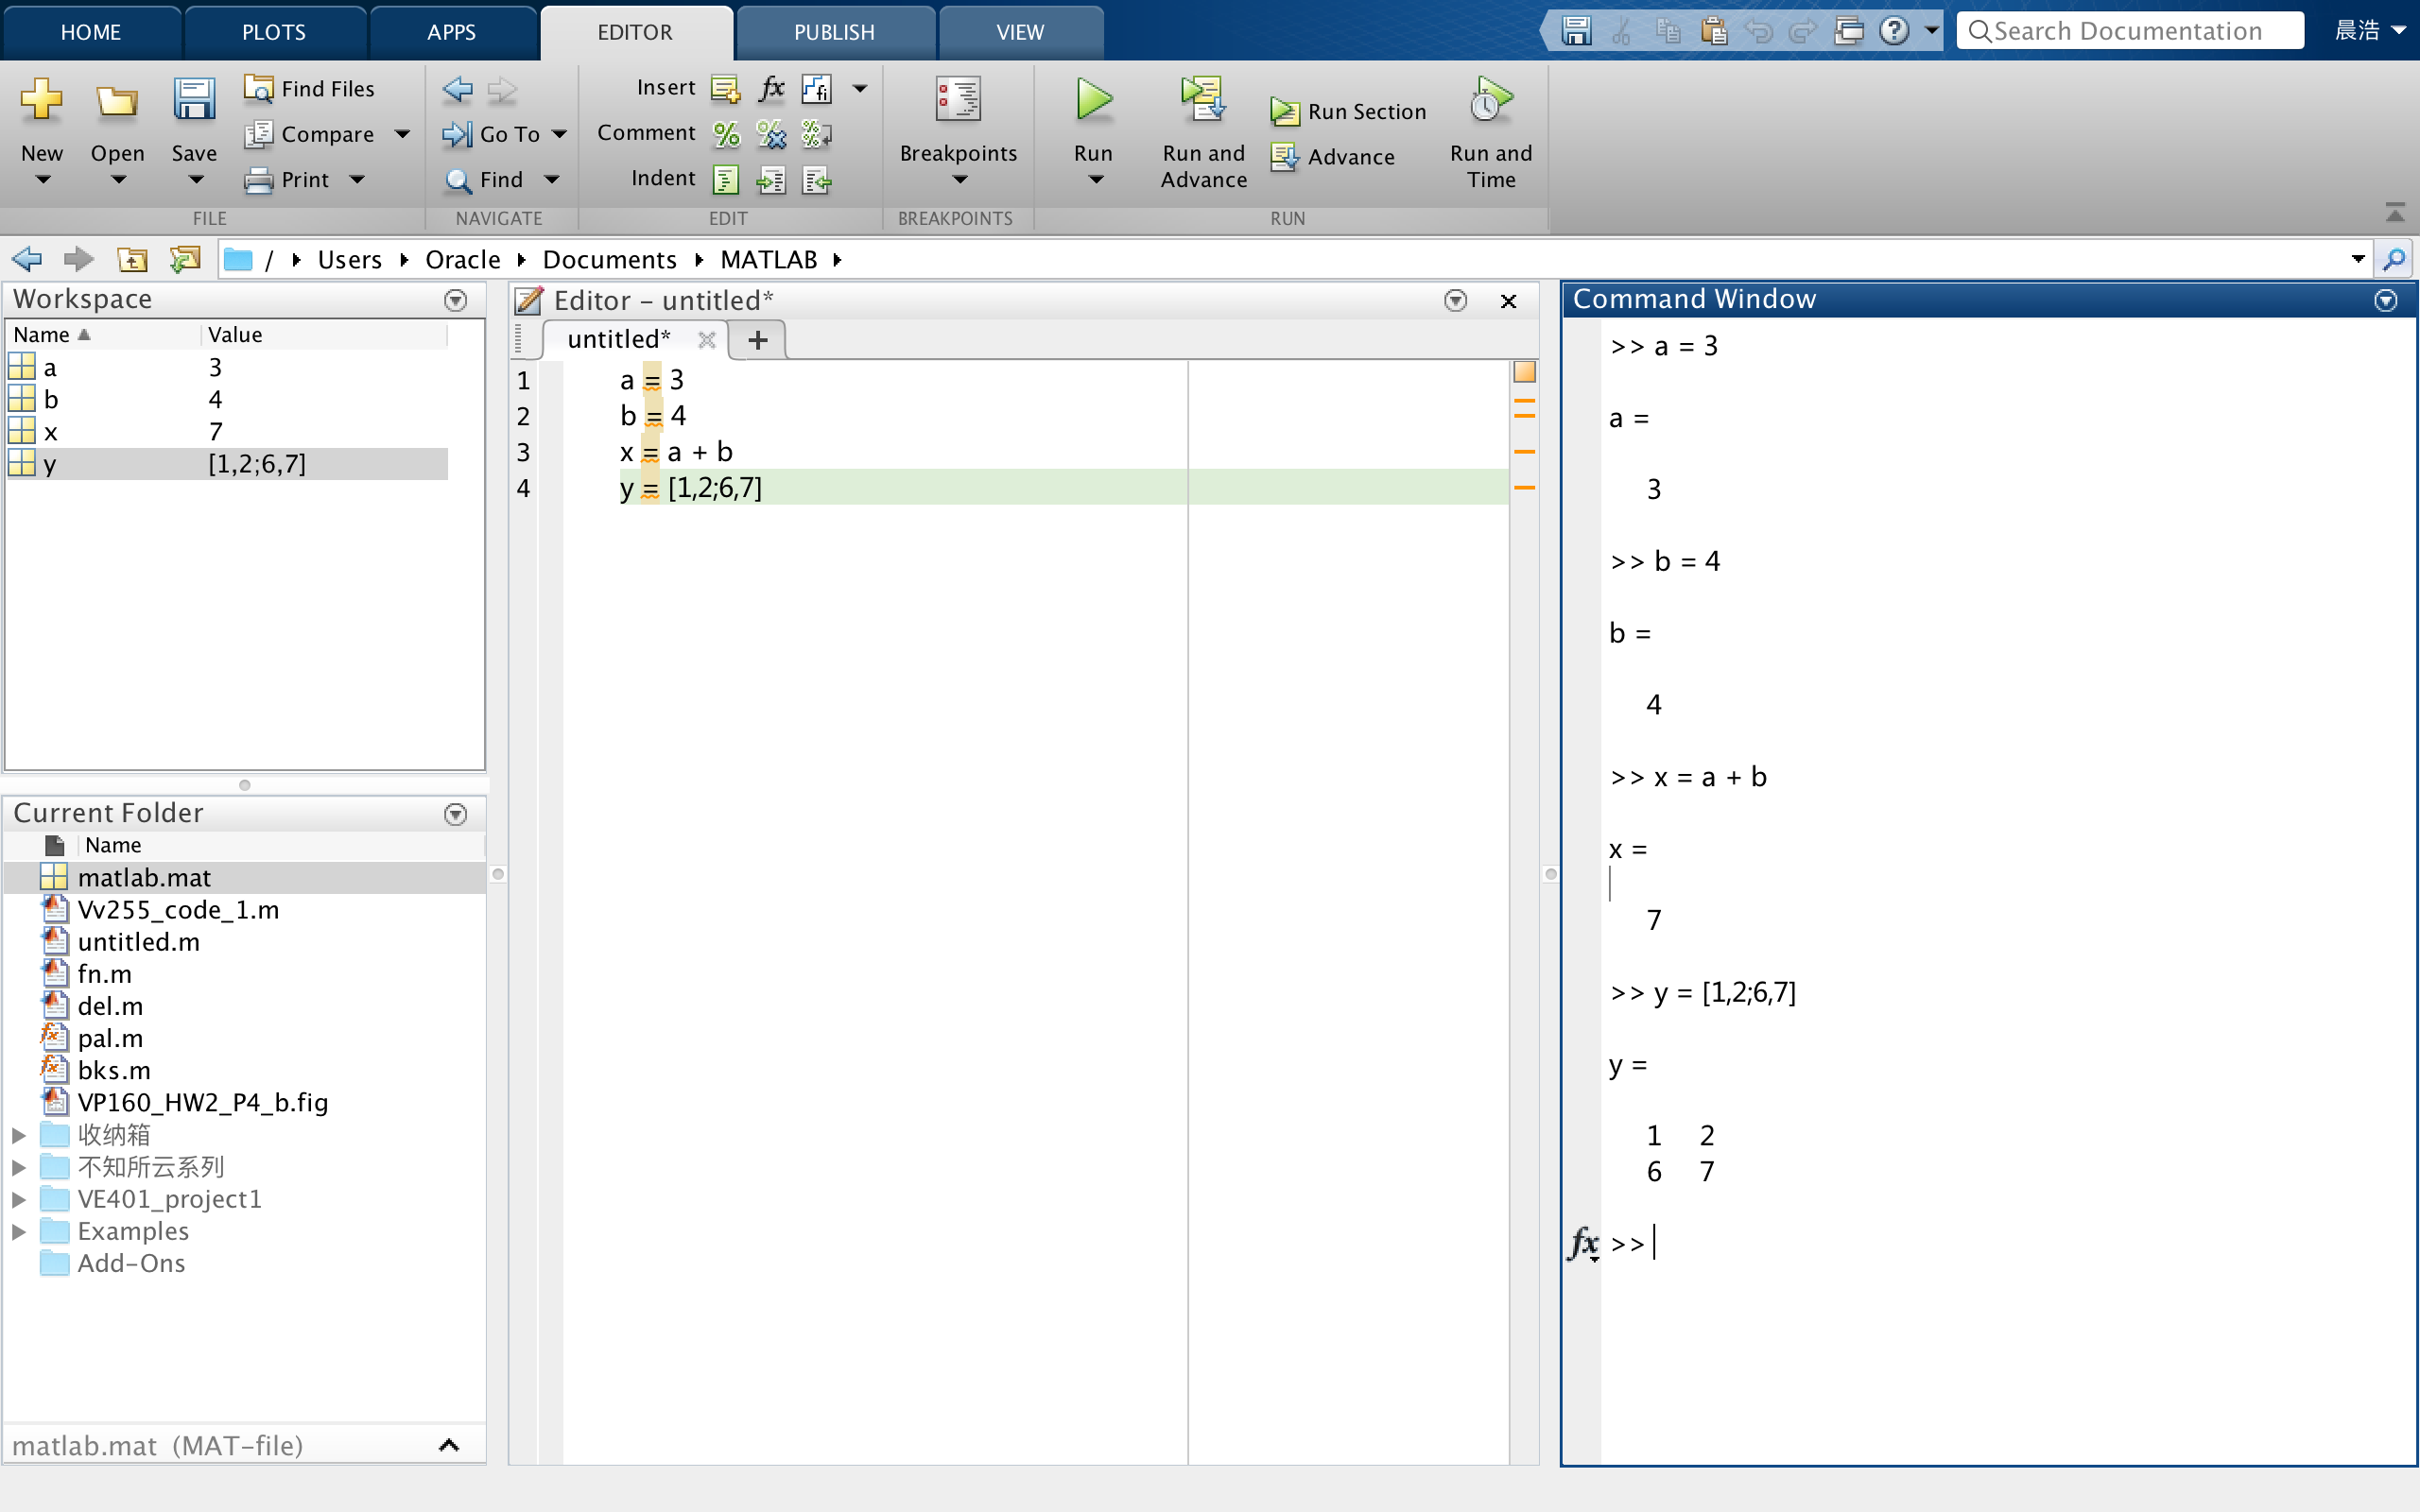
\includegraphics[width=0.95\textwidth]{window.png}
\end{figure}
\end{frame}

\begin{frame}{Interface}
\begin{block}{Workspace}
Store and show what variables are available and their value. You can double-click a variable to see its details (useful for matrix). You can also save and load workspace.
\end{block}
\begin{block}{Command Window}
Input command direct into the command line. Variables can be seen in the workspace.
\end{block}
\begin{block}{Editor}
Editor is actually where you ``buffer'' your commands. \textbf{Run} the code in the editor is equivalent to type the command line by line into command window.
\end{block}
\end{frame}


\begin{frame}{Interface}
\begin{block}{Current Folder (\& Environment)}
It indicates which folder you are currently. When you operate on file (e.g. call a function from another file), MATLAB will search the file in current directory or search path. Personally, I suggest managing your file in the current directory, which will make your life easier.

For more details about search path, you can refer to \url{https://ww2.mathworks.cn/help/matlab/matlab_env/what-is-the-matlab-search-path.html?lang=en}.
\end{block}
\end{frame}

\subsection{Syntax}
\begin{frame}{Operators \& Keys}
\begin{itemize}
\item ``+'', ``-'', ``*'', ``/'', ``.*'', ``./'', ``\^'', ``.\^'': matrix or elementwise arithmetic
\item ``='': assignment
\item ``=='': equal
\item ``\%'': comment. Will be ignored by MATLAB. Make the code easier to understand
\item ``;'': suppress output. Please add it to every line that you do not expect output! Extra output may result in dection
\item ``$\uparrow$, $\downarrow$'': view history
\item Tab: indent
\item ``clc'': clear command window
\item ``clear / clear all'': clear workspace
\end{itemize}
\end{frame}

\begin{frame}{Some Special Variables \& Constants}
\begin{block}{Tips}
\textbf{All variables in MATLAB are matrix.} Scalar is essential a $1\times1$ matix, but it allows some operations that may be invalid for a $1\times1$ matrix.
\end{block}
\begin{itemize}
\item ``ans'': default output variable; do not use ``ans'' as your own variable name in your script
\item ``i'', ``j'': virtual number
\item ``Inf'': infinite
\item ``NaN'': not a number; mostly appear when the result exceed some limit or some errors occur
\item ``pi''
\end{itemize}

\begin{block}{save \& load}
\begin{itemize}
\item save xxx: save all current variables into .mat file
\item load xxx: load .mat file; will not clear variables alread in workspace; will cover the variable in workspace if two variables share same name
\end{itemize}
\end{block}
\end{frame}

\begin{frame}{Command}
\begin{itemize}
\item ``exist'': test the existence of a varibale or a file (exist xxx)
\item ``global'': declare global variable
\item ``help'', ``doc'': show document (help xxx; doc xxx)
\item ``clc'': clear command window
\item ``clear / clear all'': clear workspace
\end{itemize}
It's good habit to add ``clc'' and ``clear'' at the first of your program, \textbf{especially in your homework}.
\end{frame}

\begin{frame}{Control Flow}
\begin{itemize}
\item if, while, for
\item while 1
\end{itemize}
\begin{minipage}{0.05\textwidth}
~\\
\end{minipage}
\begin{minipage}{0.5\textwidth}
\lstinputlisting[language=Matlab]{control_flow_demo.m}
\end{minipage}
\begin{minipage}{0.05\textwidth}
~\\
\end{minipage}
\begin{minipage}{0.35\textwidth}
Outputs: \\
1 $\hookleftarrow$ \\
2 $\hookleftarrow$ \\
3 $\hookleftarrow$ \\
4 $\hookleftarrow$ \\
look, it is a four! $\hookleftarrow$ \\
5 $\hookleftarrow$ \\
100 $\hookleftarrow$ \\
99 $\hookleftarrow$ \\
98 $\hookleftarrow$ \\
97 $\hookleftarrow$ \\
96 $\hookleftarrow$ \\
\end{minipage}
\end{frame}

\begin{frame}{Control Flow}
\begin{itemize}
\item break: break the loop
\item continue: ignore the later code in this iteration; skip directly to the next iteration
\end{itemize}
\begin{minipage}{0.05\textwidth}
~\\
\end{minipage}
\begin{minipage}{0.5\textwidth}
\lstinputlisting[language=Matlab]{break_cont_demo.m}
\end{minipage}
\begin{minipage}{0.05\textwidth}
~\\
\end{minipage}
\begin{minipage}{0.35\textwidth}
Outputs: \\
9 $\hookleftarrow$ \\
6 $\hookleftarrow$ \\
5 $\hookleftarrow$ \\
4 $\hookleftarrow$ \\
3 $\hookleftarrow$ \\
\end{minipage}
\end{frame}

\end{document}


